\documentclass[a4paper, 11pt]{article}

\usepackage[left=2.4cm, text={16.2cm, 25.2cm}, top=2.3cm]{geometry}
\usepackage[czech]{babel}
\usepackage[IL2]{fontenc}
\usepackage[utf8]{inputenc}
\usepackage{times}
\usepackage{graphicx}
\usepackage{pdflscape}
\usepackage[hidelinks]{hyperref}
\usepackage{breakurl}
\usepackage{listings}

\begin{document}

%-------------------  Titulní strana  -------------------

\begin{titlepage}
    \begin{center}{}

        \centerline{
\includegraphics[scale=0.12]{img/fit_logo.png}}

        \vspace*{\stretch{0.35}}
        {\Huge Mikroprocesorové a vestavěné systémy\,--\,Projekt} \\[1em]
        {\huge Dokumentace}
        \\[0.6em]
        \textbf{\LARGE M -- Hra na displeji }
        \vspace*{\stretch{0.65}}

    \end{center}

    {\Large 2023/2024 \hfill Dalibor Kříčka (xkrick01)}
\end{titlepage}


\tableofcontents

\newpage
\section{Úvod}
Cílem tohoto projektu bylo realizovat jednoduchou hru pro platfomormu \emph{ESP32} za použití proporcionálního
\emph{joysticku} a \emph{I2C displeje} jako vstupního a výstupního zařízrní. Hra, která byla implementovaná, je
celosvětově známá pod názvem \emph{Ping pong}. Důvodem zvolení této hry, je právě její nenáročnost na harware,
kdy je třeba pracovat pouze se třemi v čase měnícími polohu objekt a to pouze v rámci dvojrozměrného pole.


\section{Konfigurace zařízení a prostředí}
V této sekci budou přiblíženy technologie vyžity při vypracovávýní projektu a popsáno připojení periferií k zařízení \emph{ESP32}.

\subsection{Technologie}
Počet využitých technologií při vypracování této práce byl opravdu velký, proto budou níže zmíněny se základním popisem pouze
ty nejvýznamější.

\subsubsection{ESP32}
ESP32 je série energeticky nenáročných technologií soustředá na jeden čip. Disponuje 4\,MB Flash a 320\,KB RAM
pamětí a 240\,Mhz procesorem Xtensa® dual-core 32-bit LX6 microprocessor a další spoustou funkcí (např.: WiFi, Bluetooth,
I2C, UART, 34 programovatelných obecných regitrů, atd.)(více na \cite{Wikipedia:2023:ESP32}).

\subsubsection{I2C OLED displej}
Display využívá pro komunikaci s deskou rozhraní \emph{I2C}. I2C je synchronní seriové rozhraní, které využívá využivá pro komunikaci
model \emph{Master/Slave} a dva vodiče (viz \cite{Bidlo:2023:SeriovaKomunikace}):
\begin{itemize}
    \item {vodič \emph{SDA} (Serial clock) -- datový vodič,}
    \item {vodič \emph{SLC} (Data clock) -- vodič hodinového signálu.}
\end{itemize}

Displej využivá technologi OLED, která se vyznačuje faktem, že diody reprezentující černou barvu opravdu nevyzařují žádné světlo
a v podání černobílého displeje tak vytváři kontrast, který produkuje ostrý obraz i pro malá rozlišení, které je tomto
případě \emph{128x64} pixelů.


\subsubsection{Proporcionální joystick}
Joystick má v sobě zabudované 2 na sobě nezávislé \emph{potenciometry} pro každou osu (\emph{X} a \emph{Y}), pomocí kterých jsme schopni
za pomocí \emph{Analogově-digitálního převodníku} určit přesně v jaké poloze se páčka nachází. Joystick slouží zároveň také jako tlačítko.
Pro komunikaci využívá vodiče:
\begin{itemize}
    \item {vodič \emph{VRx} (Voltage Proportional x) -- napětí úměrné ose X,}
    \item {vodič \emph{VRy} (Voltage Proportional y) -- napětí úměrné ose Y,}
    \item {vodič \emph{SW} (Switch) -- stlačovací tlačítko.}
\end{itemize}

\subsection{IDF}
\emph{IDF} neboli \emph{Espressif IoT Development Framework} je prostředí pro vývoj mikrokontrolérů ESP32. Jakožto framework poskytuje
celou řadu nástrojů, knihoven a dokumentaci pro vývoj. IDF nativně podporuje \emph{jazyk C} ve kterém byl taky napsán tento projekt.

\subsubsection{Platformio}
\emph{Platformio} je vývojové prostředí, které je implementováno jako rozšíření pro aplikaci \emph{Visual Studio Code}. Jako pro jednen z mnoha
poskytuje jednotnou vývojovou platformu pro framework IDF. Umožňuje jednoduše spravovat projekty, připojená zařízení, ale také pomocí
konzolového uživatelského rozhraní nastavovat obecné registry pro periferie a tak dále.


\subsection{Zapojení a nastavení}
Zapojení bylo provedeno podle účelů jednotlivých vodičů. Na analogové registry \emph{GPIO36} a \emph{GPIO39} byly připojeny jako vstup vodiče
joysticku \emph{VRx} a \emph{VRy}. Jejich vstupní hodnoty jsou zachycovány s šířkou 12\,bitů (převáděno na hodnoty 0 až 4095). Pro tlačítko
na joysticku \emph{SW} byl použit digitální registr \emph{GPIO14} a~byl nastaven jako vstupní. Pro datový vodič \emph{SDA} a~vodič hodinového
signálu \emph{SLC} byly využity registry \emph{GPIO16} a \emph{GPIO17} a nastaveny v \emph{Menuconfig} dle zadání. Joystick
byl připojen na 3.3 Voltový zdroj. Tento zdroj byl zvolen kvůli tomu, že AD převodník je pouze 12 bitový a nedokáže tedy reprezentovat hodnotu
5000\,mV, kterou by joystick při 5\,V zdroji produkoval. Špatně by se tedy pracovalo s hodnotamy ořízlými na 4095\,mV, při kterých by
joystick přišel o téměř poloviny rozsahu v polohách od střední výchozí polohy po krajní polohu páčky.


\begin{figure}[h!]
    \centering
    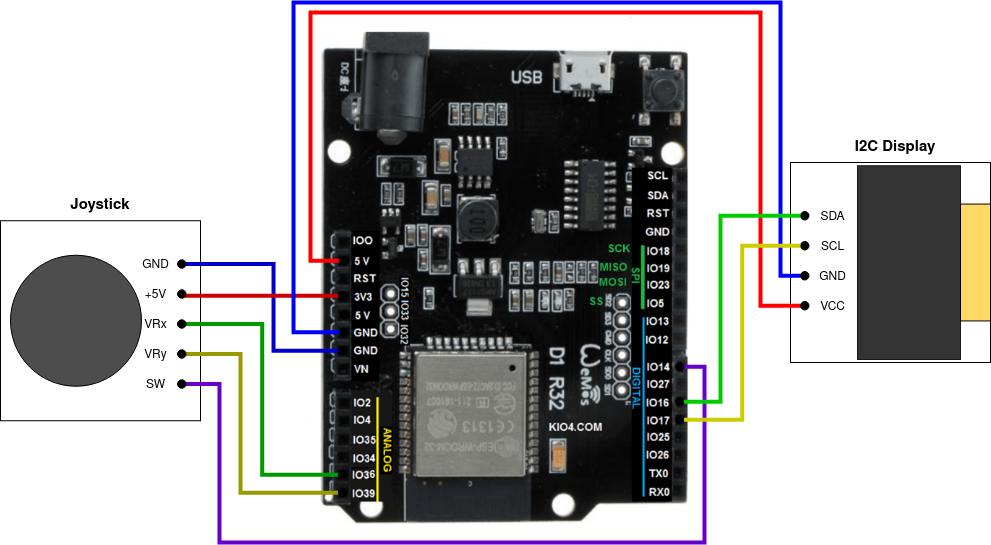
\includegraphics[scale=0.45]{img/schema_zapojeni.png}
    \caption{Schéma zapojení periferií k desce ESP32}
    \label{fig:8}
\end{figure}


\newpage



\section{Implementace}
Pro implementaci bylo využito dříve zmiňované prostředí \emph{IDF}. Pro práci s displejem byla poté využita knihovna \emph{ssd1306} a
hlavičkový soubor \emph{font8x8\textunderscore basic}. Pro čtení analogových hodnot joysticku byly využity funkce z knihovny \emph{driver/adc.h}.

\subsection{Knihovna ssd1306.h}
Knihovna \emph{ssd1306} poskytuje funkce pro jednoduché vykreslování bitmapových obrázků, textu nebo třeba linek na I2C displej. Nejvíce využívanou funkcí
byla funkce \emph{ssd1306\textunderscore bitmaps}, která umožnuje vykreslit předem definovaný bitmapový obrázek na konkrétní bod displeje definovaný souřadnicemi \emph{X} a \emph{Y}.
Dalšími hojně využívanými funkcemi byly funkce \emph{ssd1306\textunderscore clear\textunderscore screen} pro nastavení všech pixelů obrazu na černou barvu nebo funkce
\emph{ssd1306\textunderscore display\textunderscore text} pro vykreslení textu.

Všechny znaky ASCII tabulky jsou v podobě osmi Bajtových bitmapových obrázků definovány v~hlavičkovém souboru \emph{font8x8\textunderscore basic}.

\subsubsection{Vlastní úprava knihovny}
Fyzické překreslení displeje, tedy zobrazení vyrovnávácí paměti na displeji, je časově velice náročné.
Proto pro větší plynulost programu (plynulost pohybu objektů po hrací ploše), bylo potřeba z definice funkce \emph{ssd1306\textunderscore bitmaps} odstranit
zpoždění a fyzické překreslení displeje při každém využití funkce. Díky tomu bylo možné, v rámci jedné iterace herního stavu, překreslovat objekty na displeji
pouze ve vyrovnávací paměti. K pokynu k fyzickému překreslení displeje dojde vždy jednou po aktualizaci celé herní plochy.

\subsection{Herní logika}
Aby hra působila jako plynulá animace reagující na uživatelský vstup z joysticku, je třeba neustále v cyklu aktualizovat herní stav, myšleno aktualní pozice všech
pohyblivých objektů, na základě konečného počtu údálostí, ke kterým ve hře může dojít. Těmito událostmi jsou kolize míče s hráčem či horní nebo dolní hranicí, vstup
od uživatele a konec hry.

\subsubsection{Pohyblivé objekty}
Pohyb herních objektů je realizován překreslováním objektů na jiné místo v rámci herního pole v čase, tedy v jednotlivých herních stavech. Při překreslení
prvku je potřeba prvek v původní pozici nejprve smazat a až poté je možné vykresit objekt na pozici nové. Kdyby k mazaní před přesunem nedošlo, objekt by za
sebou zanechával čáru a to není žádoucí. Vzhledem k malému rozlišení displeje dochází k posunům v~rámci jednotek pixelů. Větší skoky by mohly nabourat plynulost hry.

\subsubsection{Hráč}
Hráč je herní pohyblivý objekt reprezentován bitmapovým obrázkem oddélníku a souřadnicemi X a~Y, které definují, kde se nachází levý horní roh objektu.
Hráč reaguje na polohu páčky joysticku v ose \emph{Y} pohybem nahoru a dolů. Vzhledem k tomu, že je joystick proporcionální, určuje poloha páčky, o kolik pixelů se hráč
v ose posune v daném herním stavu. Velikost tohoto skoku reprezentuje rychlost jakou se hráč pohybuje. Tímto způsobem může hráč dosáhnout třech různých rychlostí
v obou směrech.

\subsubsection{Míč}
Míč má na rozdíl od hráče, který je reprezentován bitmapovým obrázkem oddélníku a souřadnicemi polohy, definovaný navíc směr, kterým se neustále pohybuje, jak v \emph{ose X}, tak
v \emph{ose Y}. Směr je polohový vektor a~určuje tedy o kolik pixelů se posune v každém herním stavu.

Míč změní směr pokaždé při kolizi s:
\begin{itemize}
    \item {hráčem -- směru X je přiřazeno opačné číslo aktuální hodnoty směru X,}
    \item {spodní nebo horní hranicí -- směru Y je přiřazeno opačné číslo aktuální hodnoty směru Y.}
\end{itemize}
Kolize poté působí jako odraz míčku od stěny, kdy na něj nepůsobí žádná gravitace. Úhel dopadu se tedy rovná úhlu odrazu.

\subsubsection{Kolize}
K rozpoznání kolize míče s jiným objektem dochází pomocí porovnávání poloh jednotlivých objektů. Jedná li se o dvojrozměrné objekty, je třeba při kontrolách kolizí
s pravou a spodní stranou objektu přičítat k aktuální poloze taky velikost objektu. Pro rozpoznání kolize míče s hráčem je třeba porovnat polohu míče vůči hráči v obou
osách.

\subsubsection{Vstup joysticku}
Hodnota napětí, kterou na vstup joystick produkuje ve výchozí poloze, se pohybuje kolem 1790 mV (hodnota byla vypozorována). Tuto hodnotu považujeme za výhozí.
Dojde li k významnému
poklesu této hodnoty, víme že páčka byla posunuta vzhůru a že se hráč bude posunovat v ose Y vzhůru, dokud se zase neustálí kolem výchozí hodnoty. To samé, ale opačně, platí
pro pohyb směrem dolů. Dále jsou definovány jisté prahy, které jsou porovnávány s rozdílem mezi aktuální a výchozí hodnotou. Jejih postupné překračování určuje rychlost
pohybu.

\newpage

\section{Vlastnosti projektu}
Celý program je ovládán jen za pomoci připojeného joysticku, a to pohybem nebo stisknutím páčky. Po skončení kola, kdy jedním kolem je myšlena doba od záčátku
samotné hry po prohru jednoho z kráčů, je možné spustit hru znovu od začátku.

\subsection{Obrazovky}
Obsah, který je na displej vykreslován, je logicky členěn na tzv. \emph{Obrazovky}. V rámci programu je možné se setkat s následujícími \emph{třemi} druhy obrazovek:
\begin{enumerate}
    \item {\emph{Úvodní obrazovka --}}
    \begin{itemize}
        \item {zobrází se ihned po připojení mikrontroléru ke zdroji a její zobrazení trvá 5 vteřin}
        \item {po uplynutí 5 vteřin se přepne na obrazovku číslo 2}
        \item {zobrazuje informace o čísle projektu, autorovi a roku vytvoření programu}
    \end{itemize}
    \item {\emph{Obrazovka s aktivním čekáním --}}
    \begin{itemize}
        \item {zobrazuje textovou výzvu, aby bylo stisknuto tlačítko pro zahájení hry}
        \item {program je ve stavu, kdy aktivně čeká na stisk tlačítka}
        \item {po stisknutí tlačítka se přepne na obrazovku číslo 3}
    \end{itemize}
    \item {\emph{Obrazovka hry --}}
    \begin{itemize}
        \item {vykresluje samotný průběh hry}
        \item {po skončení hry se přepne zpět na obrazovku číslo 2}
    \end{itemize}
\end{enumerate}

\subsection{Průběh hry}
Po zahájení hry tlačítkem dochází k odpočtu zahájení hry, který je zobrazován ve středu obrazovky. Po odpočtu hry se dá míč do pohybu a cílem hráčů je
odrážet míč svojí postavou na soupeřovu stranu. Pokud kterýkoliv z hráčů míč v čas neodrazí (míč se dostane za hráče), tak to znamená prohru pro dáného hráče.

\subsection{Ovládání}
Hráč je ovládán pohybem páčky joysticku v ose Y. Nahnutím páčky lze dosáhnout až tří různých rychlostí pohybu hráče. Pokud je páčka ve výchozím stavu, hráč
zůstátá stát na místě. Vzhledem k tomu, že hra je určena pro 2 hráče a k dispozici je joystick pouze 1, tak dohází během hry k přepínání, který hráč je aktuálně
ovládán. Na tahu je vždy ten hráč, proti kterému se v dané době pohyhubuje míč.

\newpage


\bibliographystyle{czechiso}
\renewcommand{\refname}{Literatura}
\bibliography{manual}

\end{document}